\documentclass[a4paper, 10pt]{article}
%\usepackage{fontspec}
%\setmainfont{Lato}
\usepackage{pgf}
\usepackage{eurosym}
\usepackage{graphicx}
\usepackage{wasysym}
\usepackage{hyperref}
\usepackage{listings}
\usepackage{pxfonts}
\usepackage{verbatim}
\usepackage{color}
\usepackage{xcolor}
\usepackage{wrapfig}
\usepackage{enumitem}
\usepackage{booktabs}
\usepackage{gensymb}
\usepackage{tabularx}
\usepackage{currfile}

\hypersetup{
    bookmarks=true,         % show bookmarks bar?
    unicode=true,          % non-Latin characters in Acrobat’s bookmarks
    pdftoolbar=true,        % show Acrobat’s toolbar?
    pdfmenubar=true,        % show Acrobat’s menu?
    pdffitwindow=true,     % window fit to page when opened
    pdftitle={Assessments},    % title
    pdfauthor={Paul Vesey},     % author
    pdfsubject={Advanced Graphics Assignment },   % subject of the document
    pdfcreator={},   % creator of the document
    pdfproducer={xelatex}, % producer of the document
    pdfkeywords={'Graphics' }, % list of keywords
    pdfnewwindow=true,      % links in new PDF window
    colorlinks=true,       % false: boxed links; true: colored links
    linkcolor=violet,          % color of internal links (change box color with linkbordercolor)
    citecolor=magenta,        % color of links to bibliography
    filecolor=red,      % color of file links
    urlcolor=blue           % color of external links
}

\setlength\parindent{0pt}
\begin{document}

\lstset{language=HTML,
				basicstyle=\small,
				breaklines=true,
        numbers=left,
        numberstyle=\tiny,
        showstringspaces=false,
        aboveskip=-20pt,
        frame=leftline
        }
				
\begin{table}%
	\begin{minipage}{0.4\textwidth}%
			
\includegraphics[width=1\textwidth]{./img/LITlogo.jpg}
	\end{minipage}
	\qquad
	\centering
	\parbox{0.4\textwidth}{
		\begin{large}			
			\begin{tabular}{| r | l |} \hline
				Subject: & \textbf{Advanced Graphics}\\
								 & \textbf{\& Visualisation}\\
				Course: & \textbf{Interior Design Y3}\\
				Session: & \textbf{Autumn 2020}\\
				Lecturer: & \textbf{Paul Vesey \footnotesize{BEng, MIE, HDip}}\\
				Filename: & \footnotesize{\currfilename}\\
				\hline
			\end{tabular}
		\end{large}			
	}
\end{table}
\vspace{0.25cm}	
	
\begin{flushleft}
\Large\textbf{Assignment 3 - Masterpiece (30\%)}\\
\end{flushleft}

The concept of a masterpiece dates back hundreds of years.  A masterpiece is an object that demonstrates the skill and proficiency of its creator.  In this assignment you are going to demonstrate your mastery of Autodesk 3D Studio Max, and the V-Ray rendering engine by re-creating a single rendered image of a scene of your own creation.  Your creation is to be similar to those shown in Figures \ref{fig:1} to \ref{fig:6}.\\

The key deliverables of this project are therefore:

\begin{enumerate}
	\item Single 3D Studio Max, V-Ray Render (png or jpg of approx 4k resolution)
	\item 3DS Project folder with all files and assets included
	\item A 4 page Report on the creation of the image and the work-flow used.
\end{enumerate}

This project will take a considerable amount of time to complete.  Final renders may take over an hour to produce.  Success in this project will require an immediate start and at least 4 hours per week in addition to allocated class time.  \\

\textbf{Suggested Production Workflow}\\
Creation of images of the quality shown below requires planning and discipline in both time management and asset management.  I suggest you adopt a structured approach similar to that shown below:

\begin{itemize}
	\item Each component (asset) to be a separate 3DS file, XRefed into the 'Master' Scene.
	\item Create each asset fully, including all geometry and materials and run test renders to ensure each asset performs as expected
	\item Create an empty building model with a default material and light it  appropriately.  It is easier to light the scene when there are less objects within it.  
	\item Add the materials to the building scene.  Ensure all materials and lighting behave within expected parameters
	\item Populate the master scene with the building model and other assets and render.
\end{itemize}

\newpage
\textbf{Submission}\\

You are required to submit all assets and files used to create your scene.  This includes all materials, models, images, and other items generated.  Create a single zip file of your project folder and upload to Moodle on or before the submission date.\\


\textbf{How to Structure your Submission}
\\
All submission are to take the form of a single zip file.  The zip file must maintain the folder structure as generated by 3DS Max or Unity.   The images below, figure \ref{fig:3dsstructure} and figure \ref{fig:unity} give an indication of the folder structure that you should zip and submit.\\ \\

\begin{figure}[h]
	\centering
	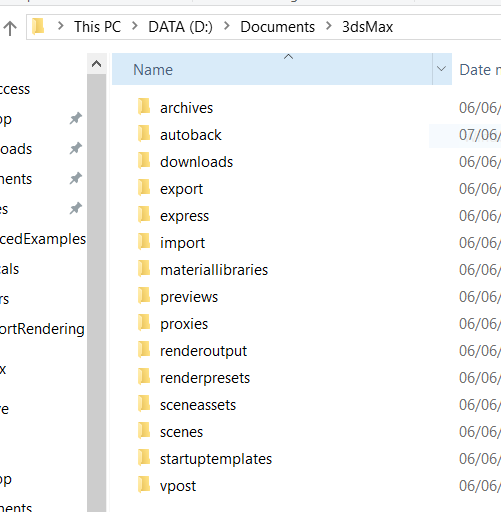
\includegraphics[width=0.5\linewidth]{img/3dsStructure.jpg}
	\caption{3D Studio Max Project Folder Structure}
	\label{fig:3dsstructure}
\end{figure}
\begin{figure}[h]
	\centering
	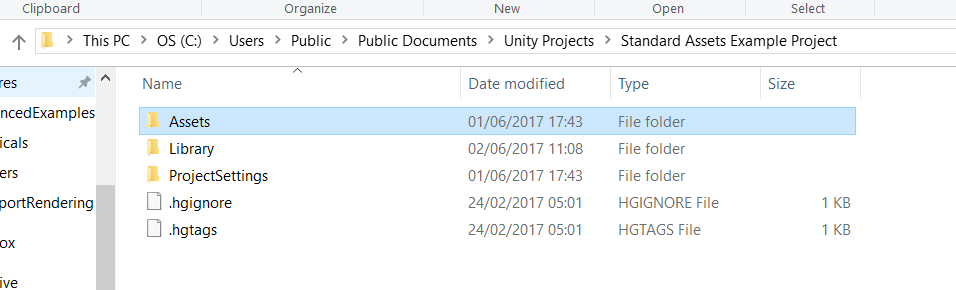
\includegraphics[width=0.9\linewidth]{img/Unity.jpg}
	\caption{Unity Game Engine File Structure}
	\label{fig:unity}
\end{figure}

All assets used during the course of the assignment are to be submitted.  All assets used and created should be placed within the appropriate folder.  To clarify, all 3ds Scene files should be placed within the 'scenes' folder; and all renders should be placed within the 'renderoutput' folder.
\\
\\
Please note that it is not appropriate to submit a single \textit{.max} file, single \textit{.jpg} file, or a single \textit{.unity} file.  

\vspace{1cm}
\textbf{Late Submission}\\
Failure to submit your assignment on or before the date and time indicated on Moodle will result in a penalty of 5\% per day or part thereof.
\\
\\
Late submission penalties will not apply in cases where a valid medical certificate is provided.  In such instances an extension of time will be granted for the duration of illness stated on the medical certificate that falls after the submission date.  A copy of the medical certificate must be included with the late submission.
\\
\\
Late submission penalties may also be avoided in exceptional circumstances.  These will be dealt with on a case by case basis.  Please note that loss of pen-drives, inability to use or access the software etc. will not be considered 'exceptional circumstances'.
\\

\textbf{Factors that will be considered when marking}\\
\begin{itemize}
	\item Realism of images
	\item Lighting
	\item Materials
	\item Composition
	\item Render errors
	\item Polygon count
\end{itemize}



\begin{figure}
	\centering
		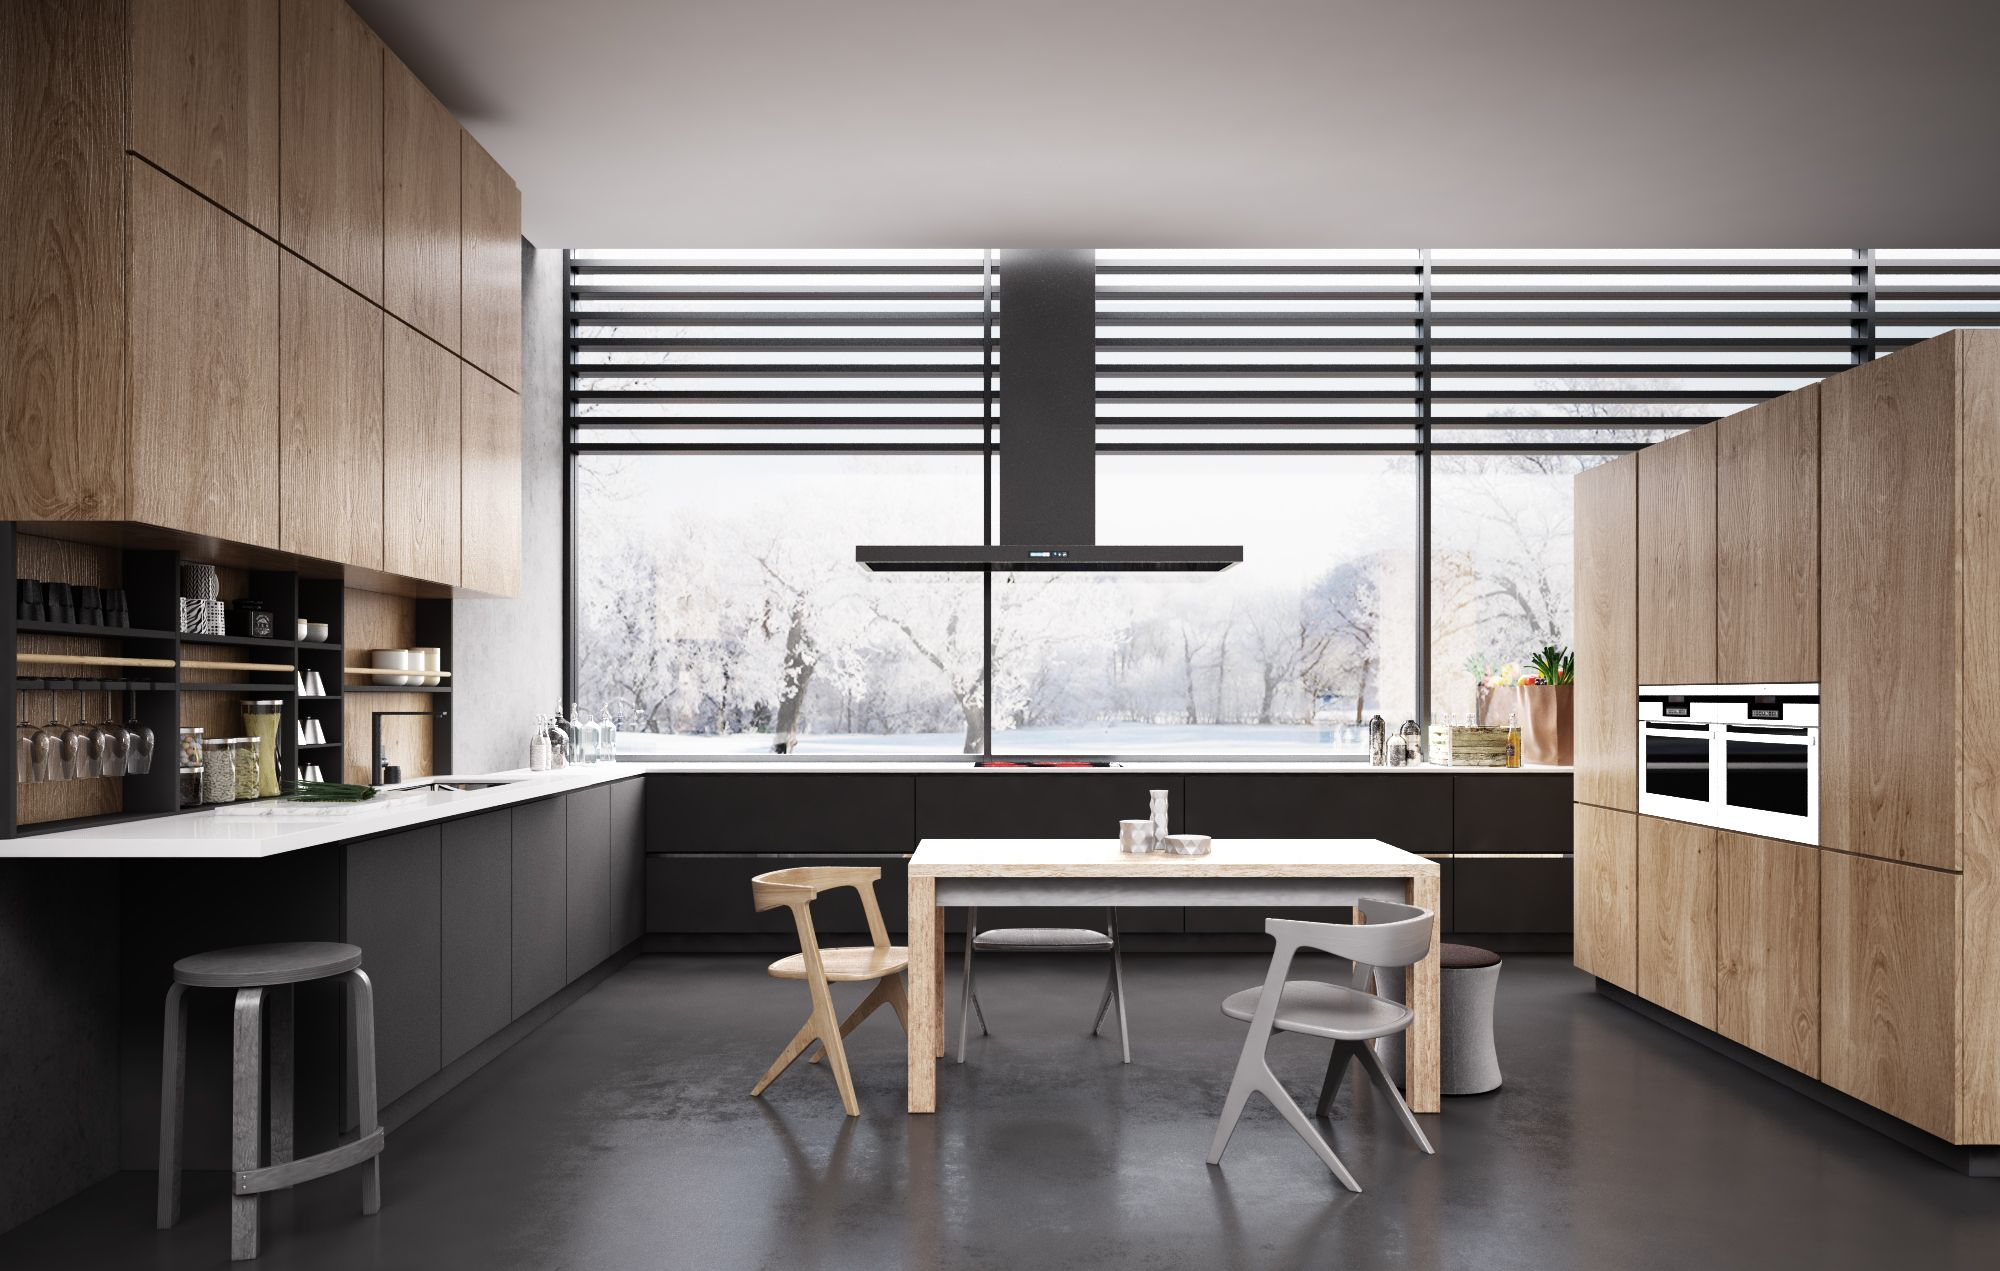
\includegraphics[width=10cm]{img/blackKitchen.jpg}
	\caption{Black Kitchen by Supardiyono Ono}
	\label{fig:1}
\end{figure}



\begin{figure}
	\centering
		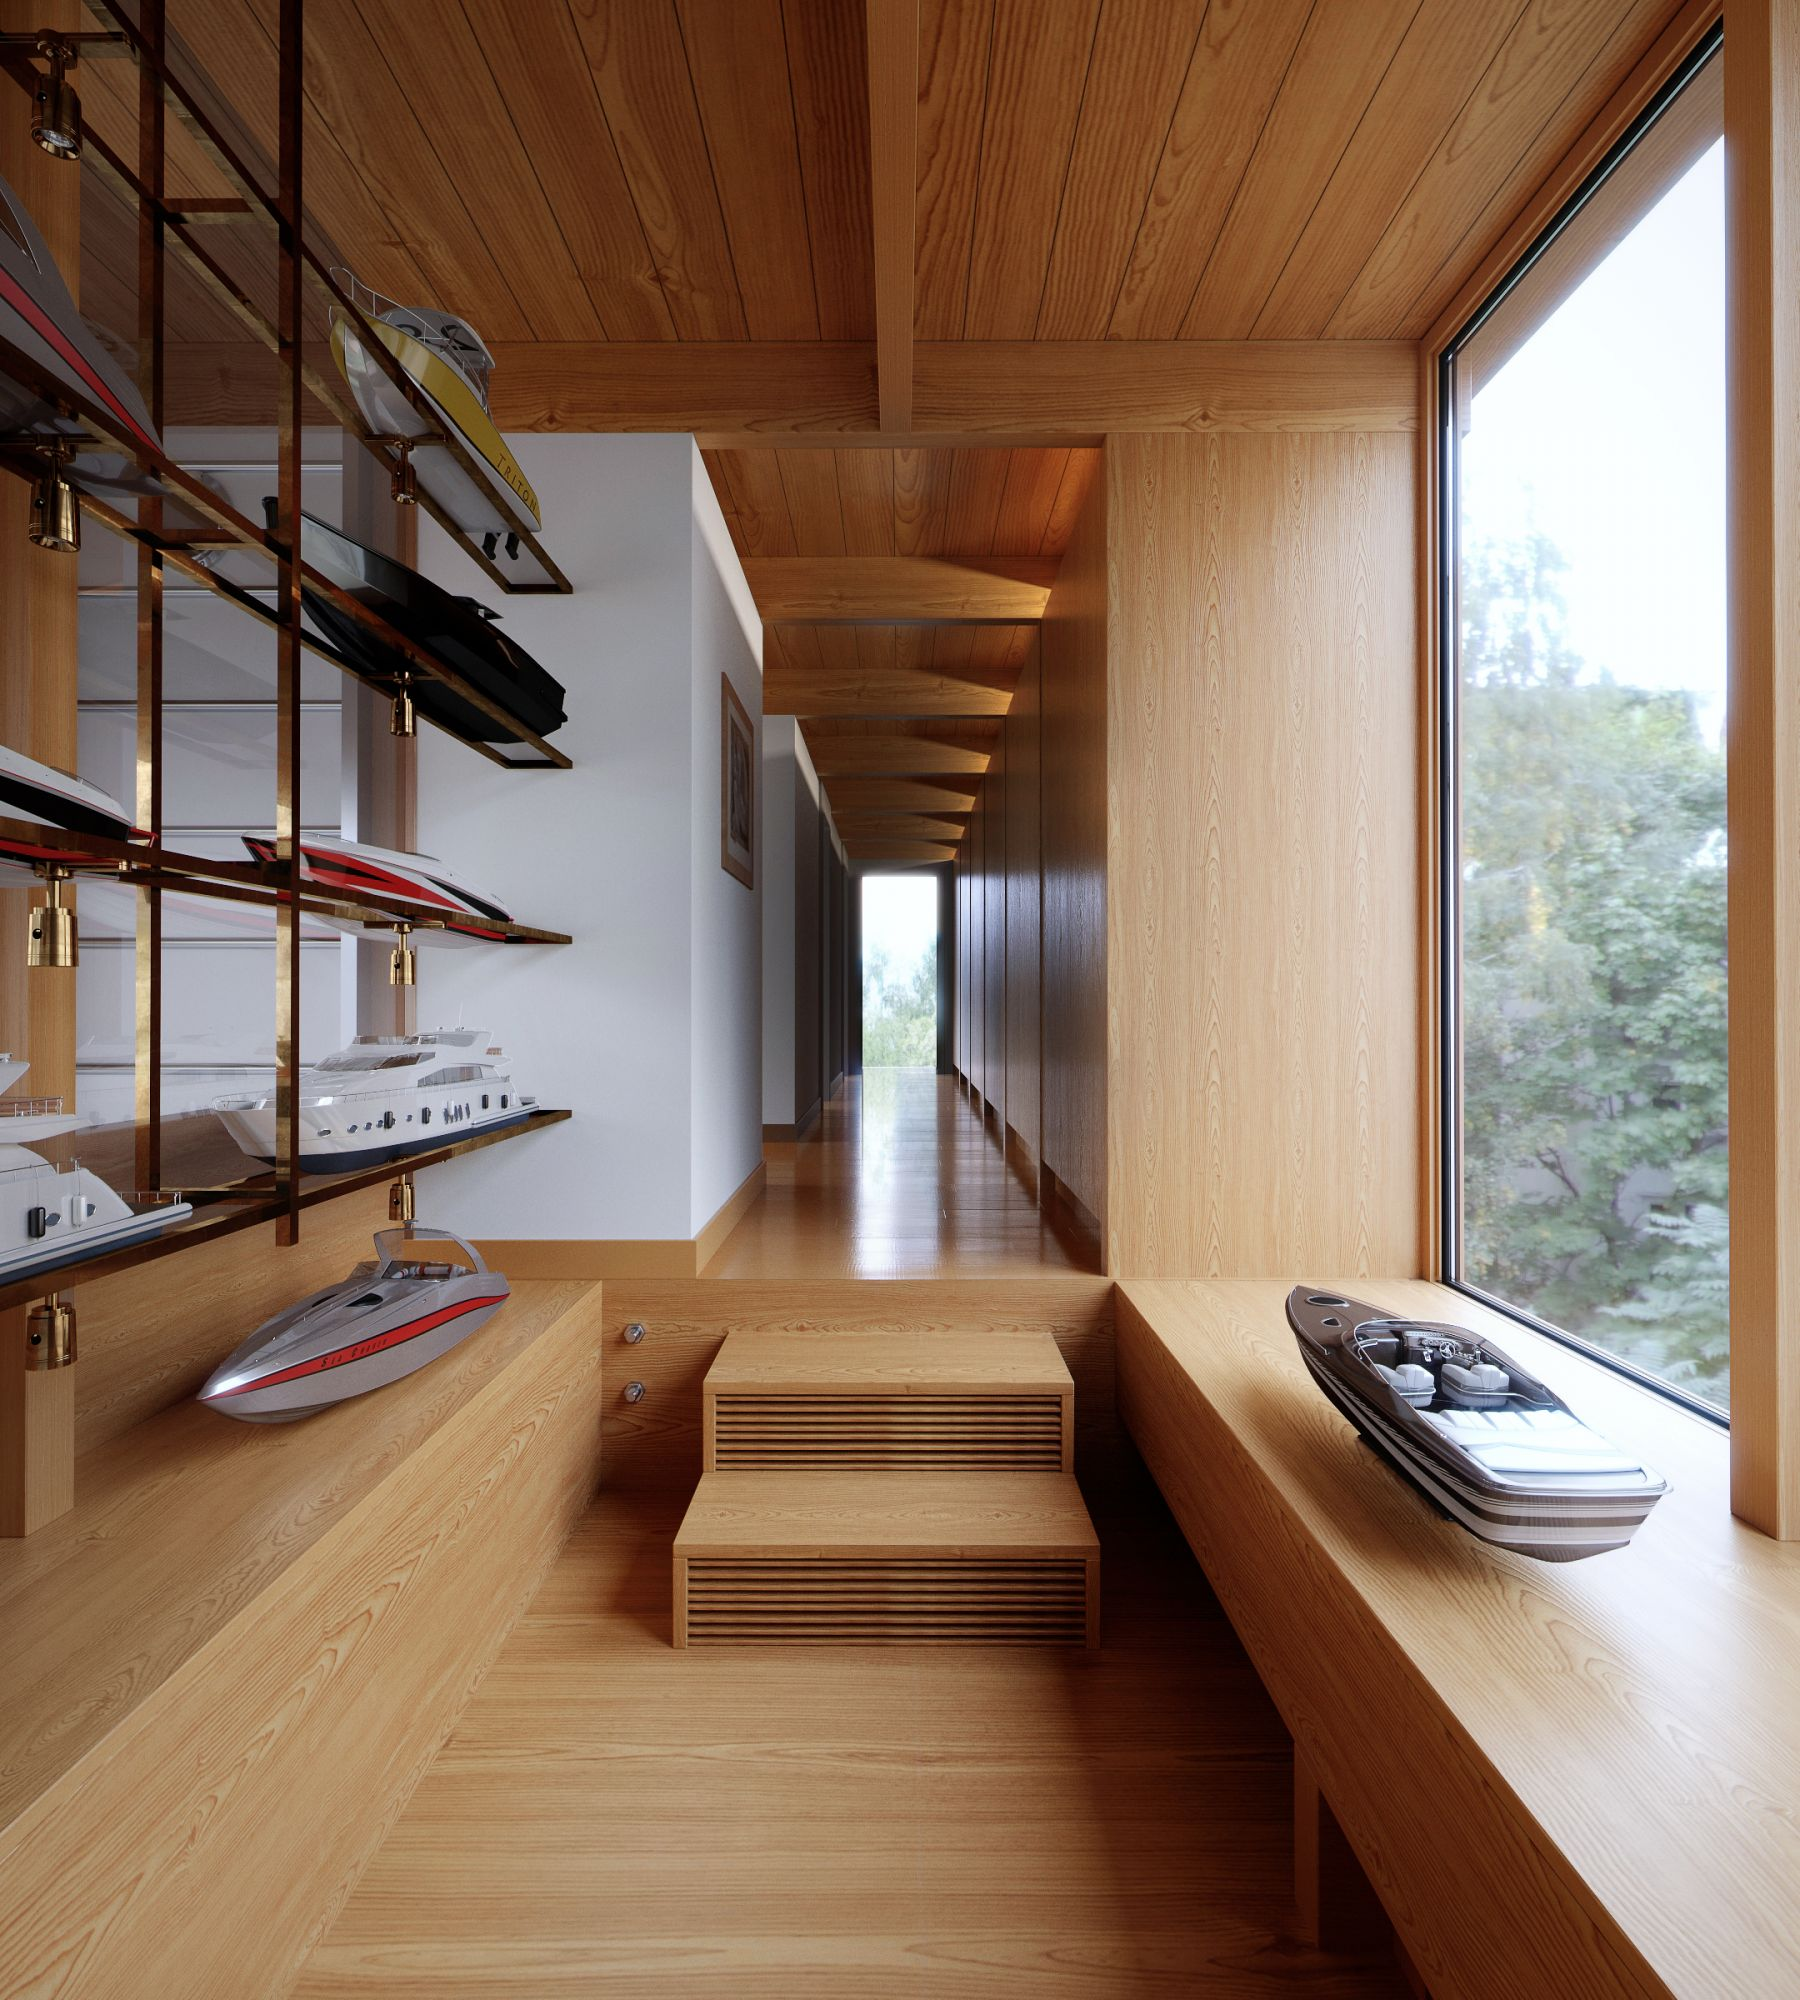
\includegraphics[width=8cm]{img/AH.jpg}
	\caption{Adpropeixe House by Bionic Digital}
	\label{fig:2}
\end{figure}


\begin{figure}
	\centering
		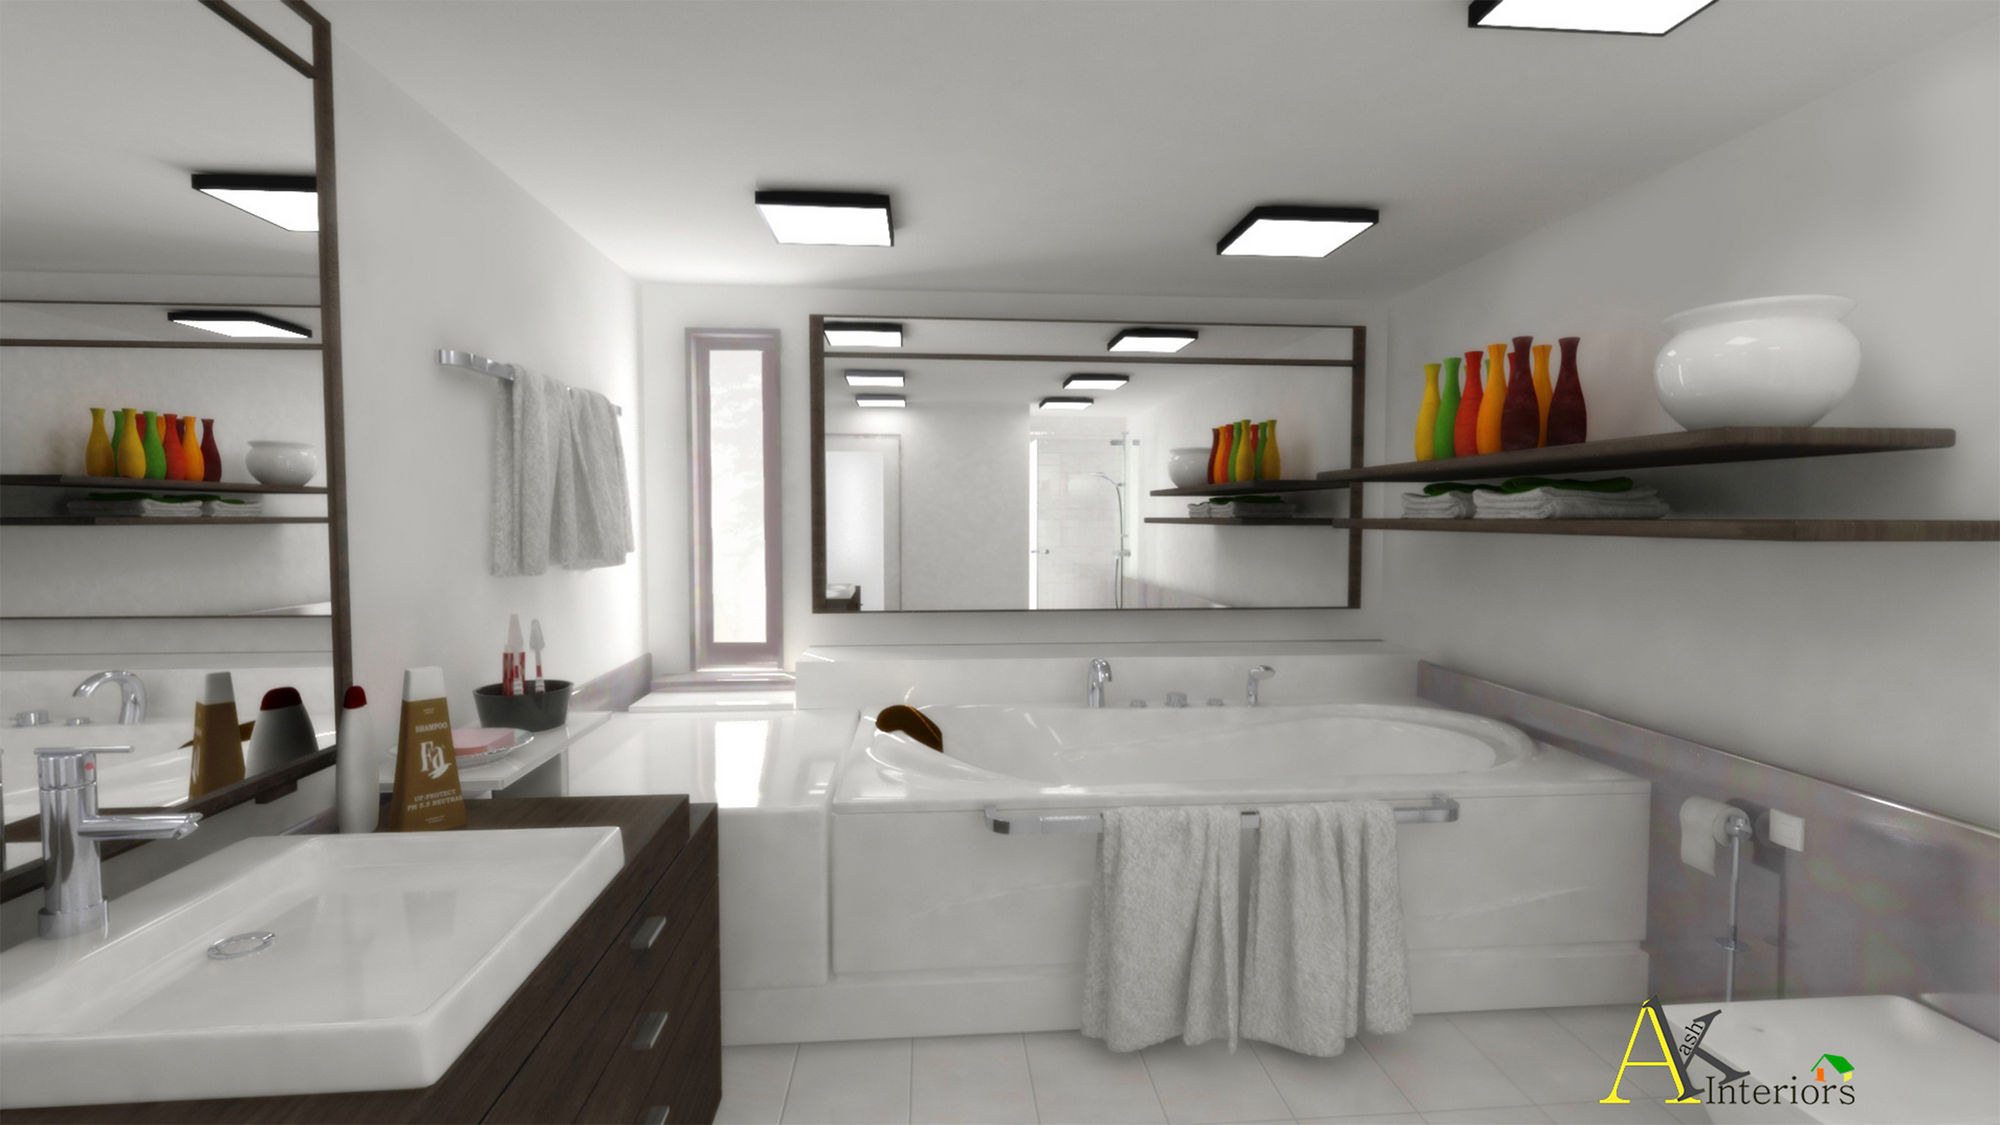
\includegraphics[width=10cm]{img/bath1.jpg}
	\caption{Stylish Bath by Aakash Prabu}
	\label{fig:3}
\end{figure}


\begin{figure}
	\centering
		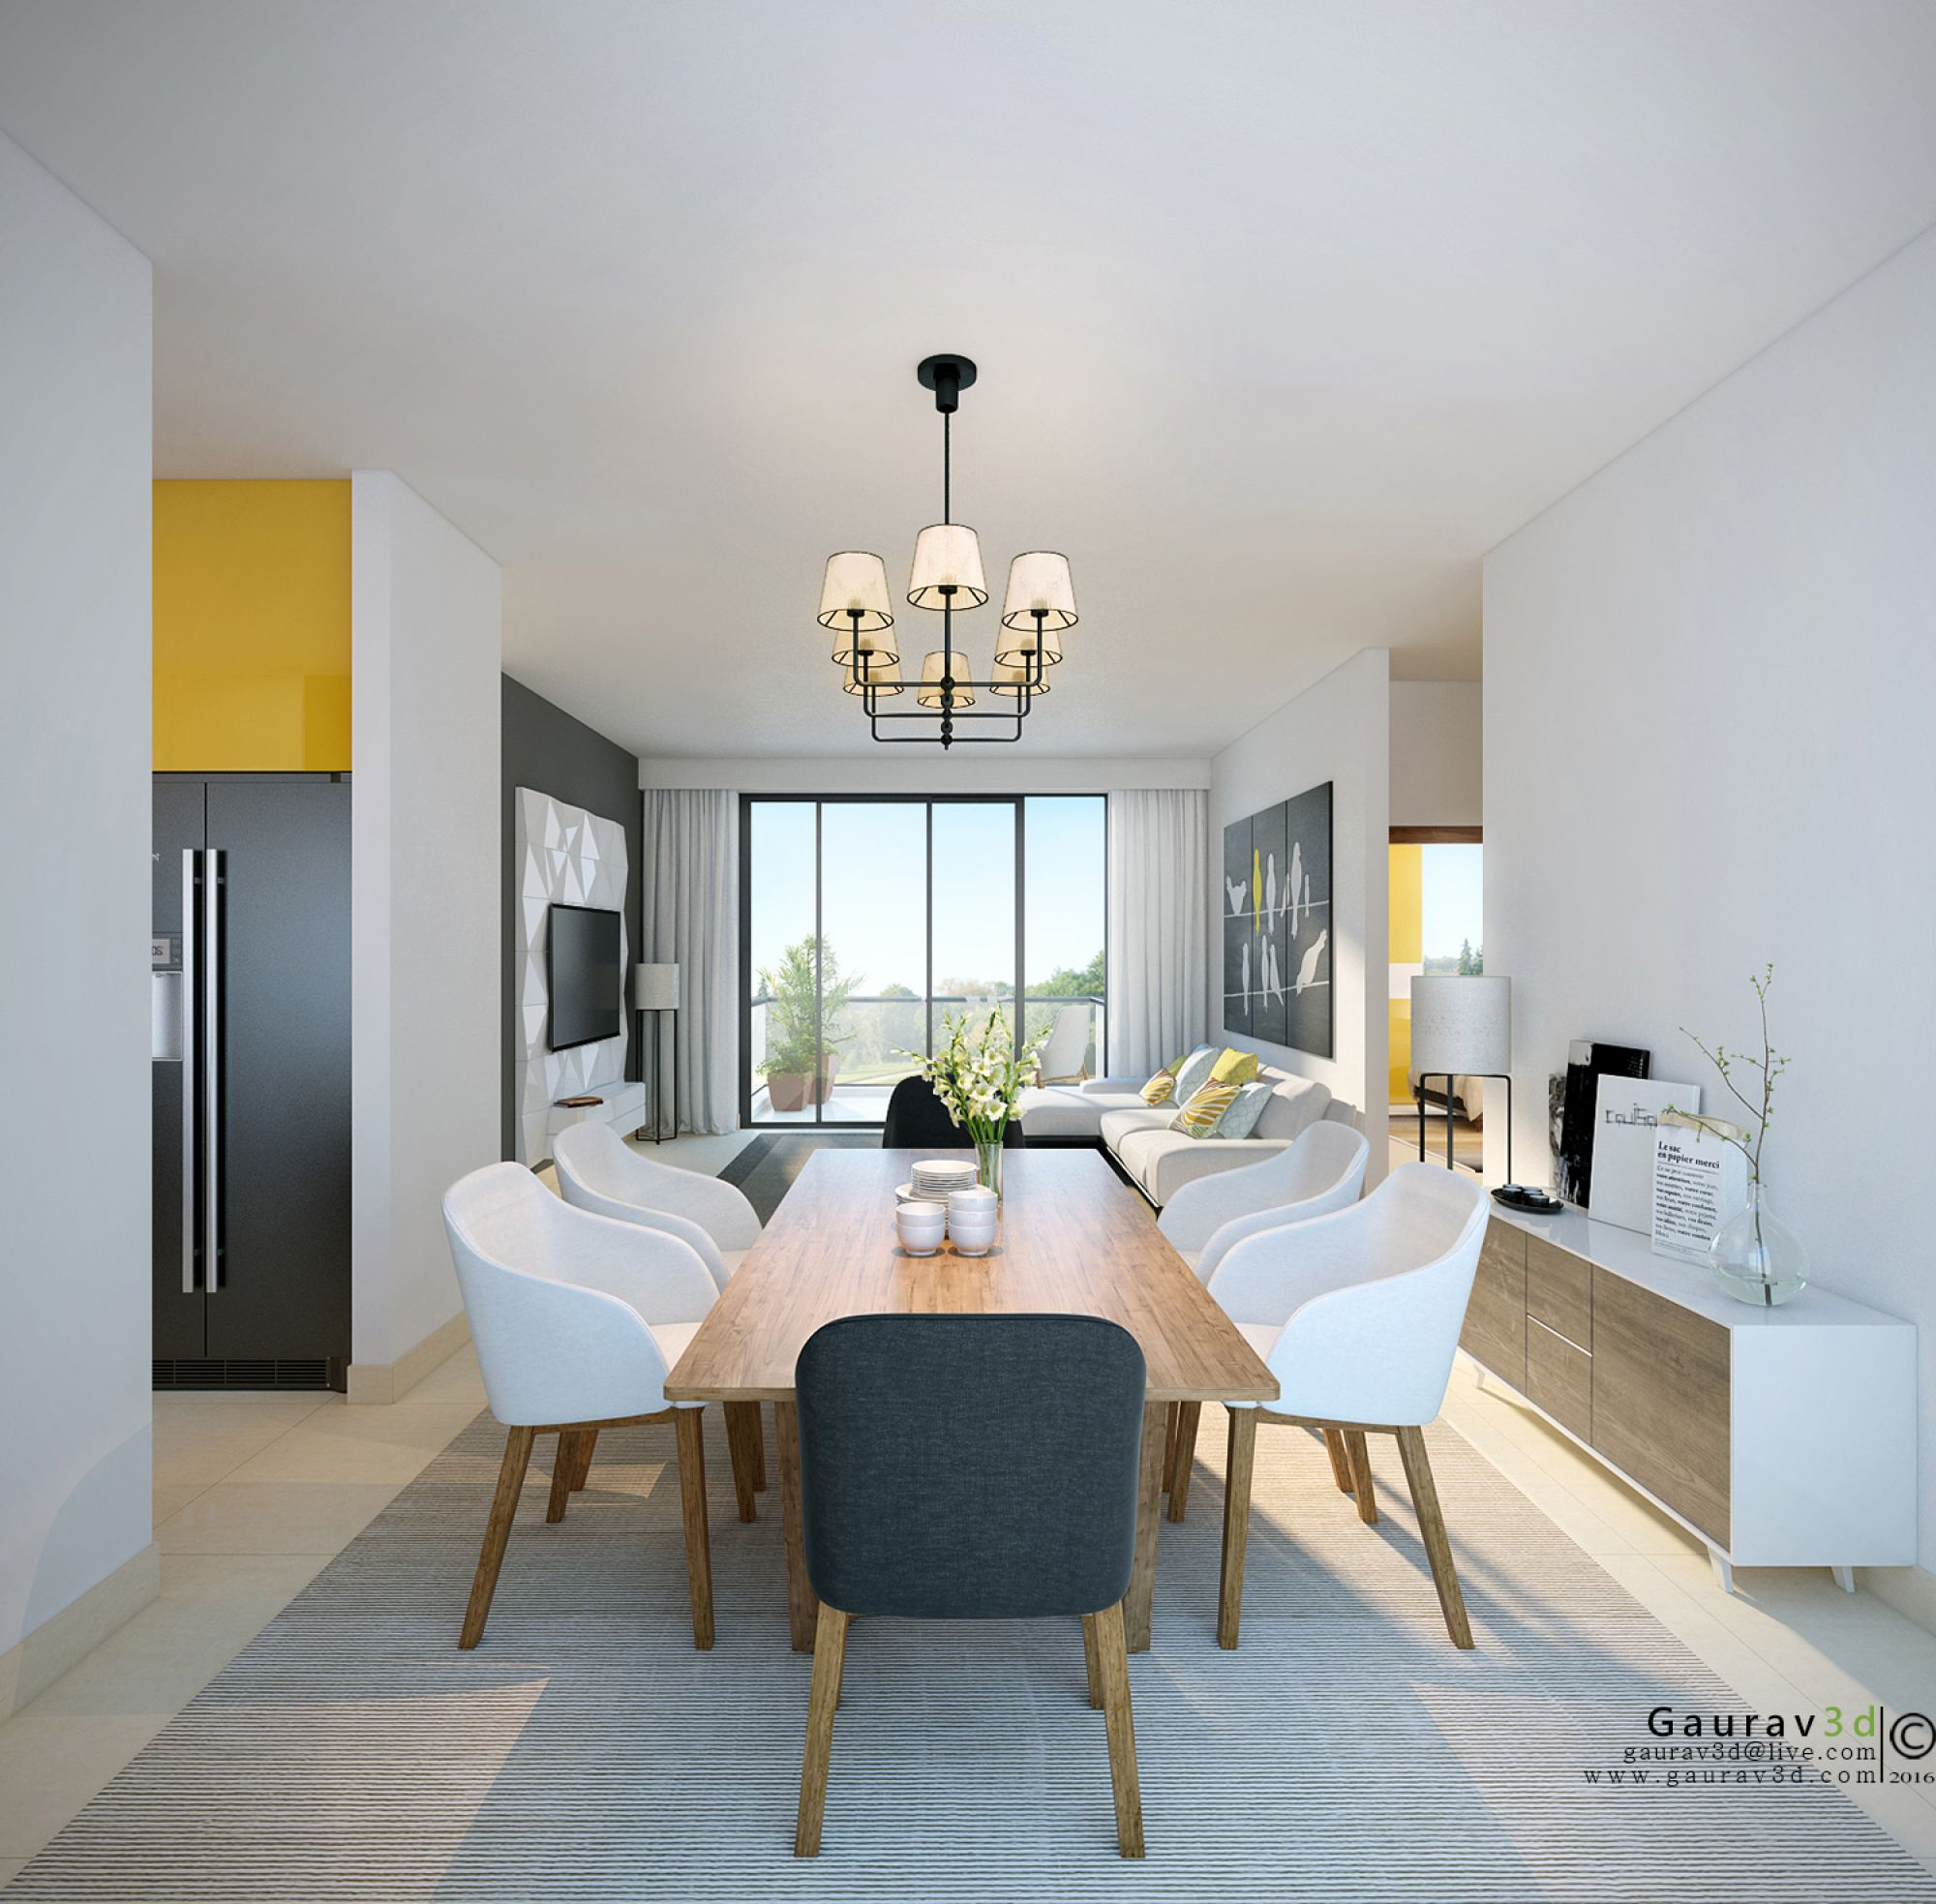
\includegraphics[width=8cm]{img/8_large.jpg}
	\caption{Living and Dining Rendering by Gaurav 3d}
	\label{fig:4}
\end{figure}



\begin{figure}
	\centering
		\includegraphics[width=10cm]{img/bedroom.jpg}
	\caption{Interior Design by Chetan Chouhan}
	\label{fig:5}
\end{figure}



\begin{figure}
	\centering
		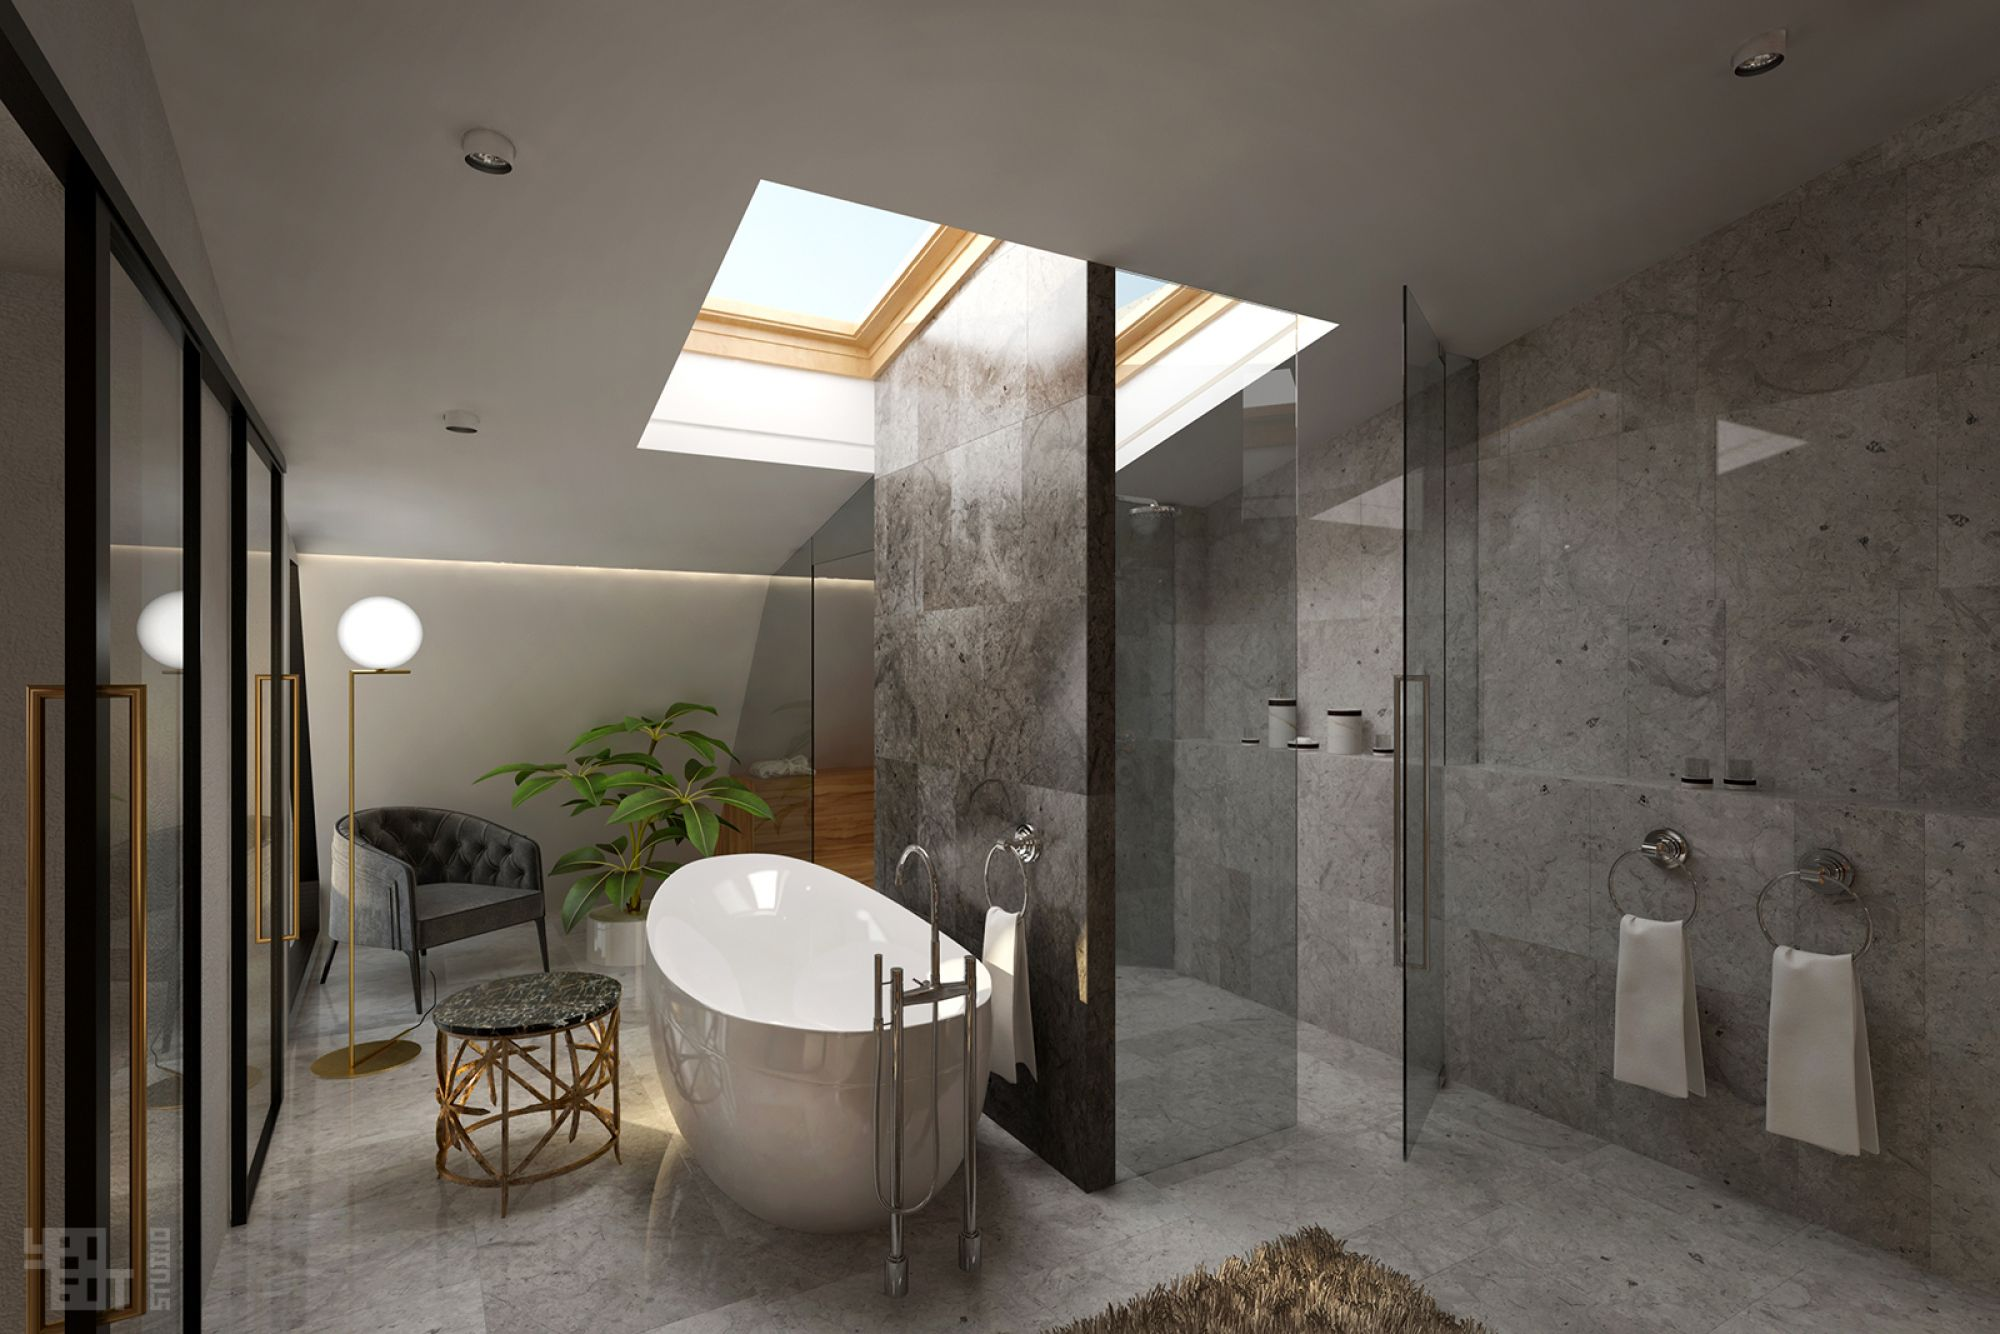
\includegraphics[width=10cm]{img/bath2.jpg}
	\caption{Bathroom Design by Uros Kovacevic}
	\label{fig:6}
\end{figure}






\end{document}